
\documentclass[10pt,journal,compsoc,twoside]{IEEEtran}

\usepackage{xcolor}

% *** CITATION PACKAGES ***
%
\ifCLASSOPTIONcompsoc
  % The IEEE Computer Society needs nocompress option
  % requires cite.sty v4.0 or later (November 2003)
  \usepackage[nocompress]{cite}
\else
  % normal IEEE
  \usepackage{cite}
\fi 


% *** GRAPHICS RELATED PACKAGES ***
%
\ifCLASSINFOpdf
  \usepackage[pdftex]{graphicx}
  % declare the path(s) where your graphic files are
  \graphicspath{{/png/}}
  % and their extensions so you won't have to specify these with
  % every instance of \includegraphics
  \DeclareGraphicsExtensions{.png}
\else
\fi


% *** ALIGNMENT PACKAGES ***
%
\usepackage{array}
% Frank Mittelbach's and David Carlisle's array.sty patches and improves
% the standard LaTeX2e array and tabular environments to provide better
% appearance and additional user controls. As the default LaTeX2e table
% generation code is lacking to the point of almost being broken with
% respect to the quality of the end results, all users are strongly
% advised to use an enhanced (at the very least that provided by array.sty)
% set of table tools. array.sty is already installed on most systems. The
% latest version and documentation can be obtained at:
% http://www.ctan.org/pkg/array

%\usepackage{mdwmath}
\usepackage{mdwtab}
% Also highly recommended is Mark Wooding's extremely powerful MDW tools,
% especially mdwmath.sty and mdwtab.sty which are used to format equations
% and tables, respectively. The MDWtools set is already installed on most
% LaTeX systems. The lastest version and documentation is available at:
% http://www.ctan.org/pkg/mdwtools







% *** Do not adjust lengths that control margins, column widths, etc. ***
% *** Do not use packages that alter fonts (such as pslatex).         ***
% There should be no need to do such things with IEEEtran.cls V1.6 and later.
% (Unless specifically asked to do so by the journal or conference you plan
% to submit to, of course. )

% specify correct hypenation here
\hyphenation{opt-ical net-orks condu-ctor accu-mulator}


\begin{document}

\title{Features Derived from Self-Supervised Representation Learning are Effective in Reverse Vaccinology}
%
%
% author names and IEEE memberships
% note positions of commas and nonbreaking spaces ( ~ ) LaTeX will not break
% a structure at a ~ so this keeps an author's name from being broken across
% two lines.
% use \thanks{} to gain access to the first footnote area
% a separate \thanks must be used for each paragraph as LaTeX2e's \thanks
% was not built to handle multiple paragraphs
%
%
%\IEEEcompsocitemizethanks is a special \thanks that produces the bulleted
% lists the Computer Society journals use for "first footnote" author
% affiliations. Use \IEEEcompsocthanksitem which works much like \item
% for each affiliation group. When not in compsoc mode,
% \IEEEcompsocitemizethanks becomes like \thanks and
% \IEEEcompsocthanksitem becomes a line break with idention. This
% facilitates dual compilation, although admittedly the differences in the
% desired content of \author between the different types of papers makes a
% one-size-fits-all approach a daunting prospect. For instance, compsoc 
% journal papers have the author affiliations above the "Manuscript
% received ..."  text while in non-compsoc journals this is reversed. Sigh.

\author{Frixos~Papadopoulos,
        Ashley I.~Heinson,
        and~Mahesan~Niranjan% <-this % stops a space

\IEEEcompsocitemizethanks{
\IEEEcompsocthanksitem F. Papadopoulos, M. Niranjan are with the Department of Electronics and Computer Science, University of Southampton, SO17 1BJ. \protect\\
% note need leading \protect in front of \\ to get a newline within \thanks as
% \\ is fragile and will error, could use \hfil\break instead.
E-mail: \{fp1n17, mn\}@ecs.soton.ac.uk.

\IEEEcompsocthanksitem A. I. Heinson is with the department of Cancer Sciences, University of Southampton, SO17 1BJ. \protect\\
E-mail: a.heinson@soton.ac.uk.

}% <-this % stops a space

\thanks{(Corresponding author: Frixos Papadopoulos.)}

\thanks{Manuscript received xxxxx xx, 2020; revised Xxxxxx xx, 2020.}

}


% The paper headers
\markboth{IEEE TRANSACTIONS ON JOURNAL COMPUTATIONAL BIOLOGY AND BIOINFORMATICS,~Vol.~X, No.~X, xxxxxx~2020, MANUSCRIPT ID}%
{PAPADOPOULOS \MakeLowercase{\textit{ ET AL.}}: Features Derived from Self-Supervised Representation Learning are Effective in Reverse Vaccinology}
% The only time the second header will appear is for the odd numbered pages
% after the title page when using the twoside option.
% 
% *** Note that you probably will NOT want to include the author's ***
% *** name in the headers of peer review papers.                   ***
% You can use \ifCLASSOPTIONpeerreview for conditional compilation here if
% you desire.


% use for special paper notices
%\IEEEspecialpapernotice{(Invited Paper)}



\IEEEtitleabstractindextext{%
\begin{abstract}
With the increasing popularity of data-driven machine learning methods, reverse vaccinology is a problem of interest. The problem is one of learning a predictor from proteins confirmed as protective antigens, and a set of non-protective antigens, with the hope of ranking novel proteins as potential vaccine candidates for experimental testing. Previous work on reverse vaccinology has used features derived from the amino acid sequence based on extracting, albeit biologically meaningful, structural and functional motifs and their distributions. Recent work in the machine learning literature has developed distributed continuous representations of amino acid sub-sequences (e.g. trigrams) in a framework of self-supervised learning. Notably, in the area of language modelling, these representations have been shown to carry context-specific semantic information. In this paper, we show that such a learned continuous representation, with its basis purely in the statistics of context, offers an effective set of features that are competitive in predictive performance with more biologically inspired ones used previously. Our work is on a small, but carefully curated, bacterial proteins dataset, and paves the way for more elaborate in-silico experiment design, and for testing the ability to extract useful information contained in biological sequences.
\end{abstract}

% Note that keywords are not normally used for peerreview papers.
\begin{IEEEkeywords}
Machine learning, Molecular biology, Natural language processing, Statistical methods.
\end{IEEEkeywords}}


% make the title area
\maketitle


% To allow for easy dual compilation without having to reenter the
% abstract/keywords data, the \IEEEtitleabstractindextext text will
% not be used in maketitle, but will appear (i.e., to be "transported")
% here as \IEEEdisplaynontitleabstractindextext when compsoc mode
% is not selected <OR> if conference mode is selected - because compsoc
% conference papers position the abstract like regular (non-compsoc)
% papers do!
\IEEEdisplaynontitleabstractindextext
% \IEEEdisplaynontitleabstractindextext has no effect when using
% compsoc under a non-conference mode.


\IEEEpeerreviewmaketitle


\ifCLASSOPTIONcompsoc
\IEEEraisesectionheading{\section{Introduction}\label{sec:introduction}}
\else
\section{Introduction}
\label{sec:introduction}
\fi
% Computer Society journal (but not conference!) papers do something unusual
% with the very first section heading (almost always called "Introduction").
% They place it ABOVE the main text! IEEEtran.cls does not automatically do
% this for you, but you can achieve this effect with the provided
% \IEEEraisesectionheading{} command. Note the need to keep any \label that
% is to refer to the section immediately after \section in the above as
% \IEEEraisesectionheading puts \section within a raised box.


% The very first letter is a 2 line initial drop letter followed
% by the rest of the first word in caps (small caps for compsoc).
% 
% form to use if the first word consists of a single letter:
% \IEEEPARstart{A}{demo} file is ....
% 
% 
% Here we have the typical use of a "T" for an initial drop letter
% and "HIS" in caps to complete the first word.
\IEEEPARstart{M}{uch} of the information about how biological function is realized is encoded in the sequential arrangement of nucleotide and amino acids in macromolecules. Though early morphological developmental processes acquiring maternal signals and epigenetic imprinting have profound effects on gene regulation \cite{genomic_imprinting_parental_influence}, the sequential arrangements of the four nucleic acids along the genome and their translation into the 20 amino acids along the length of a protein, encodes a phenomenal amount of information about cellular phenotypic behaviour \cite{durbin}. While sequences accrue variations during evolution, structural and functional properties can be conserved more robustly than the variations in sequence \cite{variation_prot}. It is also the case that sequence is more easily determined by experimental techniques than either molecular structures or their precise biological function \cite{lee_redfern_orengo_2007}. Yet, we have detected only a small portion of the proteome and its respective function or structure \cite{dark-proteome1} \cite{dark_proteome2}. Consequently, inference from biological sequences using statistical and machine learning techniques can be very powerful and has received much attention in research \cite{durbin} \cite{pellegrini_2016}. Predicting secondary structures of proteins \cite{jpred4} \cite{Ni}, grouping proteins into families \cite{dani} \cite{pfam}, predicting interactions between proteins \cite{prot-interaction} and their subcellular localization \cite{prot-Subcellular} \cite{psortb} are some examples of this endeavour. 

From a machine learning perspective of tools used in such biological sequence analysis, insights and algorithms derived from \textit{Natural Language Processing} (NLP) \cite{nlp_fundamentals} have played a big part in early phases of development. These included the use of hidden Markov models (HMM) for representing families of proteins and stochastic context-free grammars for analysing RNA folding \cite{durbin}. With the advent of high throughput measurements from transcriptomic and proteomic technologies, classification \cite{haussler-pnas-paper}, clustering \cite{spellman} and outlier detection algorithms \cite{gunawardana_outlier} from statistical machine learning have been popular tools. More recent developments in machine learning with deep architectures \cite{deep-genomics-review} \cite{barash_splicing} \cite{jaganathan_2019} have shown the power of extracting useful representational space from biological data, in which clustering and classification problems become easy tasks.

An integral element of the development pursued in this paper is the idea of \textit{self-supervised learning} \cite{representation-learning}, with its roots in computer vision \cite{imagenet_2015} and NLP \cite{nlp_fundamentals}. In self-supervised learning with NLP, we note that sentences in a language are arranged in a semantically meaningful way, and the context in which words and phrases of a sentence appear carries good information to learn representations \cite{representation-learning}. By training a deep neural network to predict the context in which parts of the input appears, we end up with semantically rich representations of that input. In natural language processing, the Word2Vec \cite{mikolov2013-original} representation of words, which are built from a deep network that maps words as symbolic tokens to continuous-valued distributed representations, has proved to be enormously powerful \cite{mikolov2013_2nd}. Encouraged by this, several communities have developed distributed vector representations in their domains of applications (dna2Vec \cite{dna2vec}, ProtVec \cite{protvec}, mol2vec \cite{mol2vec} and node2vec \cite{node2vec}). In particular, the ProtVec representation has been used with success on several biological problems \cite{protvec} \cite{tape}, such as in understanding new antibiotic-resistant proteins \cite{tape}.

In this work, we borrow the ProtVec representation of trigrams of amino acids and seek to deploy this in a problem of inference from protein sequences. The inference problem we consider is whether we can classify a given protein as an effective vaccine candidate or not, also tested in \cite{heinson_2017}\cite{heinson_2019} \cite{dalsass_2019}. This is a Reverse Vaccinology (RV) problem \cite{moxon_2019} \cite{vernikos_medini_2014} which is of global importance, as it is related to the improvement of vaccines and the discovery of new ones against diseases that have an unmet need, or against novel pathogens. Using machine learning over filtering approaches to this problem, allows for considering the entire bacterial proteome for identifying effective vaccine candidates and not only extra-cellular proteins \cite{vaxijen_2007} \cite{bowman_2011}. It has been shown that proteins of other subcellular localisations can be effective vaccine components as well \cite{nebenzahl_2007} \cite{fritzer_2010} \cite{henningham_2012}. In our earlier studies, a Support Vector Machine (SVM) was used to classify the 400 protein sequences of the BPAD200 dataset \cite{heinson_2017}, achieving an Area-Under-the-Curve score (AUC) of 0.79 \cite{heinson_2017}. A recent extension \cite{heinson_2019} used the BPAD200 dataset again to show that a relatively simple Logistic Regression (LR) classifier performed nearly as well (AUC=0.74) as the more complex SVM from the earlier study \cite{heinson_2017} and a Random Forest (RF) classifier \cite{heinson_2019}. In these earlier studies \cite{heinson_2017} \cite{heinson_2019} described above, a large number of features (525) are extracted from each protein sequence by running annotation tools that predict various aspects of biological function, along with uncertainties in them. This is a commonly adopted strategy to map from variable-length sequences to a fixed dimensional vector space in which classic machine learning algorithms can be applied \cite{dalsass_2019}. The important point here is that these tools aim to predict some specific biological property such as sub-cellular localization or hydrophobicity, and are often chosen on that basis. Also, sometimes no appropriate biological tools can be found for inference on organisms such as bacteria \cite{heinson_2019}. In contrast, sequence representations learned in a self-supervised manner are designed to extract context-based features in a purely statistical setting \cite{protvec}.  

In this work, we explore how features derived from protein sequences using biological tools, as carried out in earlier studies, compares with features taken from Prot-Vec \cite{protvec}, a self-supervised representation learning setting. In both cases, we carry out dimensionality reduction using clustering and principal component settings. We show that the purely statistical technique of representation learning, which is based only on the primary protein sequence, offers features that are competitive in performance in this task. This is important because the ProtVec features are derived from considering context alone in a broad setting across a large database of protein sequences (UniProt \cite{uniprot_2018}), with no reference to the specific problem of reverse vaccinology being addressed.
	
A particular difficulty in formulating RV problems for machine learning is the construction of datasets. Unlike in high throughput measurements on the omic scales \cite{haussler-pnas-paper} \cite{spellman}, the number of candidate proteins experimentally confirmed as vaccine candidates is very small \cite{dalsass_2019}. Further, for the same reason, constructing a negative dataset is difficult. The most accurate RV bacterial proteins dataset we have at present in the literature is the BPAD200 dataset \cite{heinson_2017}, constructed by careful curation of the literature and used previously by \cite{heinson_2017} \cite{heinson_2019} \cite{dalsass_2019}, which is used in this work and also made available as supplementary material to this paper. 

The remainder of the paper is organised as follows: in section 2 of the paper, we describe the methods used; following this, section 3 presents the empirical results obtained; a discussion of the results and some general directions arising from this is given in section 4, and a summary of conclusions are given in section 5.


%METHODS----------------------------------------
%\ifCLASSOPTIONcompsoc
%\IEEEraisesectionheading{\section{Methods}\label{sec:methods}}
%\else
\section{Methods}
\label{sec:methods}
%\fi

\subsection{Summary of the Dataset}
\label{sec:methods1}


Since the construction of the BPAD200 dataset has been described previously \cite{heinson_2017}, we give only a succinct summary here. "A Bacterial Protective Antigen (BPA) was identified as a protein that led to significant protection (p $<$ 0.05) in an animal model (i.e., bacterial load reduction or survival assay) following immunisation and subsequent challenge with the bacterial pathogen" \cite{heinson_2017}. The BPA was only termed a BPA if two independent researchers agreed that it had met this definition. The curation of these BPAs was undertaken utilising the google scholar search terms: “Potential Vaccine Candidate”, “Protective antigen”, “Bacterial Vaccine Candidate”, “Bacterial Vaccine Antigen”, “Bacterial Protein Antigen”, “Novel Vaccine Candidate”, “Bacterial Vaccine Candidate”, and “Vaccine Candidate Mouse”. The curation effort searched through the first ten result pages for each one of these terms. The negative training data (non-BPAs) was assembled by randomly "selecting a protein from the same bacterial species and subcellular localization as each BPA" \cite{heinson_2017}. Following this, "non-BPAs were discarded and re-sampled if they matched a BPA with $>$ 98\% similarity" \cite{heinson_2019} (using BLASTp \cite{blast}). Additionally, to ensure as diverse a set of training data as possible they were also discarded and re-sampled if they matched an already selected non-BPA with an e-value $<$ 10x10^-3\cite{heinson_2017}\cite{blast}.


\subsection{Model construction}
\label{sec:methods2}

We constructed and compared several classifiers, developing approaches to optimally exploit features derived from self-supervised learning. To this end, we utilised the 100-dimensional representations of the 8000 trigrams published by the authors of Prot2Vec \cite{protvec}. Our models were: (a) a baseline SVM classifier, which represented each of the proteins in a 100-dimensional space obtained by summing the representations of all overlapping trigrams that occurred on the protein sequence, following what we regard as a naïve approach similar to Mofrad & Asgari \cite{protvec}; (b) a reduced dimensional feature representation, obtained by standardising (mean-centring, unit variance) the representations used for (a) and Principal Component Analysis (PCA) of the standardised 100-dimensional space, with a set threshold of 94.5\% variation to select the number of principal components used; (c) a histogram of templates (HoT) representation, obtained by clustering the 8000 100-dimensional trigrams into a number of clusters (tuned between 20-200), and counting the number of occurrences of trigrams when assigned to their nearest cluster centres, in a manner identical to how such representations are constructed from low level image features for computer vision \cite{bovw-computer-vision}. For the HoT representation (c) we also compared normalised histograms in place of counts (i.e: vector elements sum to 1), and tf-idf (Term Frequency, Inverse Document Frequency) normalization as used in classic text processing \cite{tf-idf}. We combined the representations (b) and (c), using Support Vector Machines (SVM), Random Forests (RF), eXtreme Gradient Boosting (XGBoost) and Logistic Regression (LR) classifiers. Identical to the setting of Heinson et al. \cite{heinson_2017}, we used nested ten-fold cross-validation (n10CV) to evaluate generalisation performance and compare the models constructed. Where relevant, grid search was used for hyper-parameter tuning. 


\subsection{Evaluation}
\label{sec:methods3}

The optimal model after model selection went through evaluation tests to measure the statistical significance of its predictive ability in a robust way. The main methods used were Leave-One-Bacteria-Out-Validation (LOBOV) and error analysis. LOBOV was followed as in past studies where it was first introduced \cite{heinson_2019}, and measured the generalized predictive ability of the optimal model on novel bacteria proteomes. Error analysis involved testing whether there are any consistent insights about the predictions made by the best models (including the optimal) or about the BPAD200 dataset itself.


\section{Results}
\label{sec:Results}

\subsection{Baseline model}
\label{sec:baseline}
The baseline support vector machine classifier (linear kernel), with input the 100-dimensional Prot2Vec representation obtained by summing the trigram vectors, required substantial computational time to be trained and had a performance of AUC=0.60 (std. dev. 0.08 across cross-validation runs). We inspected the distribution of the resulting vector representations and found them to be non-Gaussian, with features biased towards large values for longer proteins, simply as a consequence of having a larger number of trigrams.


\subsection{Performance of Classifiers}
\label{sec:pca-hc}

Feature reduction was carried out by Principal Component Analysis (after standardising the baseline vectors)  to deal with the curse of dimensionality \cite{dynamic_programming}, the length bias on the distribution of the protein representations, as well as reducing the complexity of classifiers. As shown in fig. \ref{fig:fig-pca}, much of the variance was captured in low dimensions with the first two principal components accounting for 42\% and 23\% respectively. The first 11 principal components accounted for 94.5\% of the variance. 

The results showed that the first 2 PCs (principal components, fig. \ref{fig:fig-pca}) and the first 5 PCs account for 65\% and 85\% of the variation in the dataset, respectively. We further observed that six proteins appeared to be outliers in the distribution of the data in the feature space defined by the first 5 PCs: YP\_008168905.1 (non-BPA), YP\_177962.1 (non-BPA), YP\_001331790.1 (BPA), AAA20874.1 (BPA), NP\_345151.1 (BPA), CAA63564.1 (BPA). Amongst those outlier proteins, the SasC protein from Staphylococcus aureus (NCBI-Protein ID: YP\_008168905.1 \cite{YP_008168905.1}) was in the set of 48 proteins that were consistently misclassified from selected models and during LOBOV (see section  \ref{sec:lobov}), and is also the most conserved protein in BPAD200.

\begin{figure}[!t]
\centering
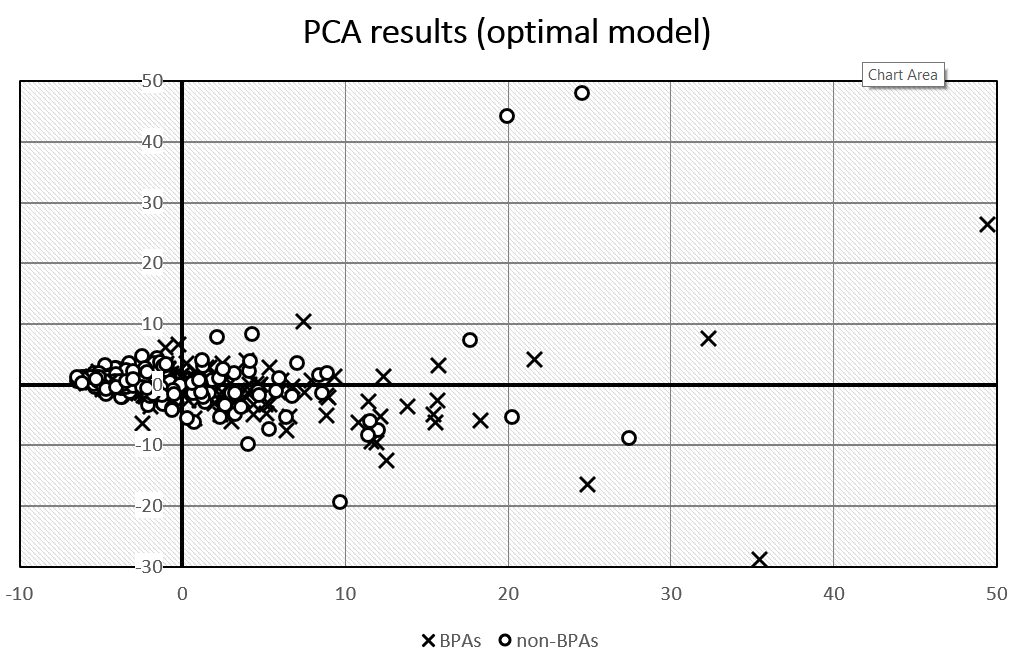
\includegraphics[width=3.2in,height=2in]{png/papad1.png}
\caption{Projection of the 100-dimensional protein trigram representations on two dimensions. The first two principal components account for 42\% and 23\% of the variance. PCA-based reduction gave a low dimensional feature space and improved classification accuracies, in combination with simple logistic regression classifiers (see fig. \ref{fig:fig-model-selection})}
\label{fig:fig-pca}
\end{figure}

\textcolor{red}{Considering hierarchical clustering in isolation, the best dataset was constructed with 20 clusters, with silhouette score = -0.03. The silhouette scores of all clustering runs were near zero and this was not ideal, because it indicated that overlapping clusters of trigrams were obtained from hierarchical clustering. Despite low silhouette scores, classifiers trained on HoT vectors generated from the hierarchical clustering results performed well (see fig. \ref{fig:fig-model-selection}), which confirmed that following a bag-of-word approach improves on the baseline results and reduces the noise present in the protein vectors.}

Fig. \ref{fig:fig-model-selection} shows the performance of selected classifier-feature combinations in comparison to the naïve baseline model. We note that the approaches based on dimensionality reduction along the various lines of principal component projections and histogram bag of features following clustering, give a significant increase in overall performance in comparison to the naïve use of learned representations (the baseline). We should also note that, while these are in the same rough league of performance, the purely statistical approaches do not outperform the more biologically informed features considered earlier \cite{heinson_2019}.

\begin{figure}[!t]
\centering
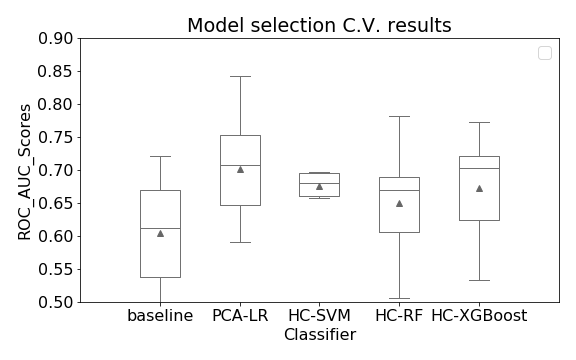
\includegraphics[width=3in,height=2in]{png/papad2.png}
\caption{Performance of various classifiers on bacterial antigen prediction. Different approaches to dimensionality reduction improve classification accuracies, in comparison to the naive method of averaging trigram features obtained by self-supervised learning along the length of each protein. Uncertainties (box plots) are obtained in nested ten-fold cross-validation. Triangles are mean AUC values.}
\label{fig:fig-model-selection}
\end{figure}

Monitoring the performances during the cross-validation loops we observed consistent low performance for fold #3. Such abnormal performance when partitioning the data suggests the influence of outliers in the data. When outliers are present in the test set, their contribution to reduced performance is limited (i.e. number of outliers), whereas when outliers are in the training partition, they have the potential to produce poor models affecting test set performance to a significantly greater extent. The next section gives results of systematic error analysis and LOBOV. The best performing was the PCA-LR model \ref{fig:fig-model-selection} and was chosen for analysis using LOBOV. The values of the tuned hyper-parameters for the optimal model were: C=0.01. It is also noted that using just the first PC from the dataset visualised in fig. \ref{fig:fig-pca}, which accounts for 42\% of variation in the original dataset, for input to an LR classifier gives a cross-validated AUC score of 0.64 (std.dev: 0.08). This highlights again the efficiency of the optimal model for inferring the BPA signal of a protein.

\begin{figure}[!t]
\centering
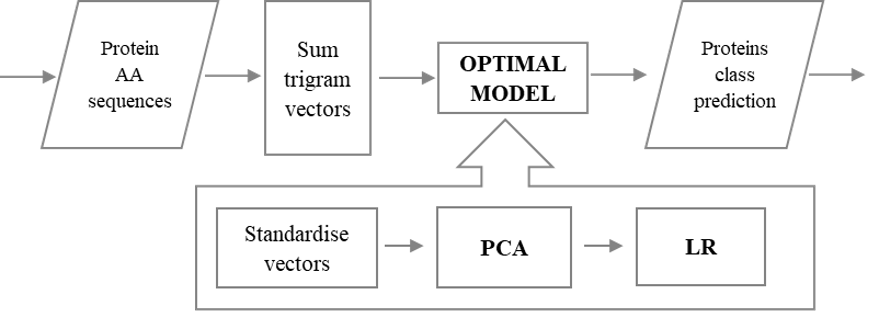
\includegraphics[width=3in,height=1.1in]{png/papad3.png}
\caption{Flowchart for the final RV pipeline, including the optimal model selected. The figure demonstrates the simple and fundamental statistical methods used by the model produced, despite the difficulty of the task of classifying proteins into BPAs and non-BPAs.}
\label{fig:fig-pipeline-diagram}
\end{figure}



\subsection{Evaluation}
\label{sec:evaluation}

\subsubsection{LOBOV}
\label{sec:lobov}

Leave-One-Bacteria-Out-Validation (LOBOV) was performed using the configurations of the optimal model (standardisation-PCA-LR) and according to the procedure explained in section \ref{sec:methods}. Fig. \ref{fig:fig-lobov} shows the performances in each bacterial species using the statistical model explored in this work compared against the same published by Heinson et al. \cite{heinson_2019} from a more biological knowledge-driven feature set. On fig \ref{fig:fig-lobov}, the LOBOV AUC scores of the model produced in this study for some species (Leptospira interrogans, Salmonella enterica, Yersinia pestis) were below 0.5 and were changed to their complement values (=1-score) on the plot. The same was done for the AUC score for Chlamydia trachomatis reported by Heinson et al. \cite{heinson_2019}. 

Against each of the performance bars in fig. \ref{fig:fig-lobov}, we have also included the number of proteins available in the dataset taken from that bacterial species. We checked if the difference in performance across different species could be due to sparsity in data and found a slight negative correlation of the test size with the AUC score across the species (Spearman corr=-0.33). We do not take this to be a strong conclusion.

\begin{figure}[!t]
\centering
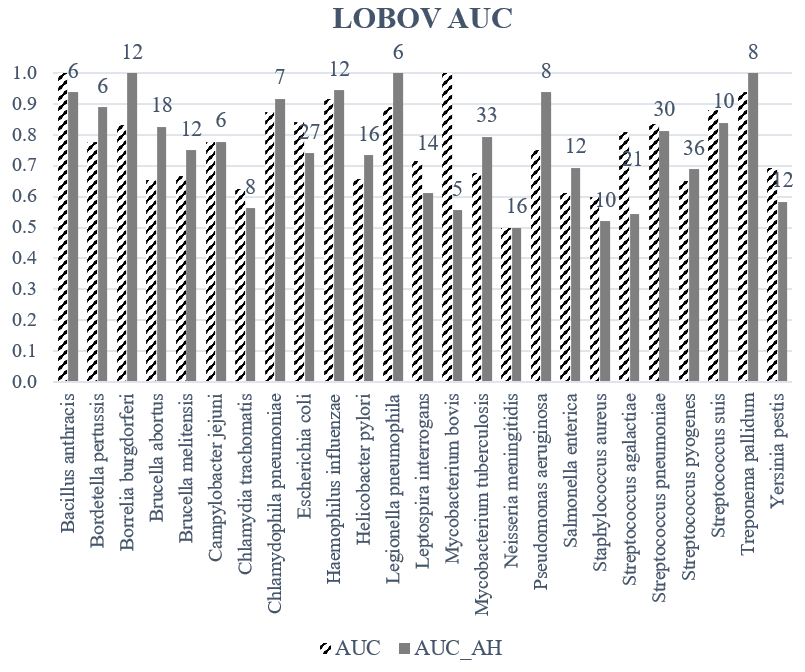
\includegraphics[width=3.4in,height=3.1in]{png/papad4.png}
\caption{Variation in classification performance on proteins taken from different bacterial species. LOBOV AUC scores obtained in this study (protein features derived from self-supervised learning) are compared against the similar study of Heinson et al. \cite{heinson_2019} which was based on biologically meaningful feature sets. Test set sizes are shown above each bars pair for each species. Dark bars are for LOBOV results of Heinson et al. \cite{heinson_2019}.}
\label{fig:fig-lobov}
\end{figure}

\subsubsection{Further Error Analysis}
\label{sec:lobov}

We looked for outlier proteins on which the classifiers made errors consistently. By retraining the selected models (fig. \ref{fig:fig-model-selection}) with the same partitions of training and test sets, we identified 54 proteins that were misclassified by all models. 48 of these 54 were misclassified during LOBOV analysis as well. Taken together, these suggest that differences in performance across different models is not randomly distributed and the antigenic properties of some proteins are harder to predict than of others. A multitude of molecular reasons may exist for this, such as the rarity of peptides that could be recognized by the immune system, triggering the correct immunological response. We observe that the constructed dataset is insufficient to undertake a detailed analysis at the level of peptides. Also, it was suggested that the models struggle more with classifying non-BPA proteins correctly, as 28/48 non-BPAs and 20/48 BPAs were misclassified. This is not necessarily unexpected as it is much more difficult to generate a negative training dataset of non-BPAs that completely represent the entire proteome of bacterial species. 

\textcolor{red}{Looking in more detail at the misclassified BPAs and the relevant literature, there is varying evidence about the antigenicity of the protein 1DI0\_A (NCBI-Protein ID \cite{1DI0_A}). This is discussed more in the discussion section. 1DI0\_A was the top result \cite{heinson_2017} of a BLASTp \cite{blast} search against the Ref-Seq NCBI DB (database of non-redundant protein sequences \cite{ncbi-prot-nr-db}), where the ‘18-kda Brucella cytoplasmic protein’ reported by \cite{goldbaum_velikovsky_1999} was used as the query. The BLASTp result was re-produced in this study with a 98.73\% similarity between the two proteins and e-value=4e-110. When this alignment was reproduced, it was observed that there are different amino-acids at 2 positions on each sequence and each of them was indicated as a conservative substitution by the BLASTp tool. 1DI0\_A is involved in the process of biosynthesis of riboflavin, an important vitamin in microorganisms \cite{riboflavin}. Its subcellular localisation is reported to be cytoplasmic \cite{psortb}, it was reported to be a lumazine synthase after laboratory experiments \cite{goldbaum_velikovsky_1999} and it is a product of the BLS gene \cite{BLS}.}


\section{Discussion}
\label{sec:Discussion}

The results show that features derived from self-supervised learning, a purely statistical method that extracts continuous distributed representations of data based on the context in which they appear, are competitive with knowledge-driven features extracted, in solving a specific inference problem in biological sequence analysis, that of selecting candidate BPAs. The continuous search for novel vaccines in the light of the rapid emergence of anti-biotic resistance by pathogens \cite{who_antibiotic_resistance} will be facilitated by such computational advances. It is important to make four observations here. 

First, the best performing model in the present work, which consisted of PCA reduced features paired with logistic regression classification (PCA-LR, section \ref{sec:model-selection}), achieves an AUC score of 0.70 (std.dev: 0.07), which is competitive with the best-published results of 0.79 on the same dataset \cite{heinson_2017} \cite{dalsass_2019}. The methods we apply on the baseline vector representations (section \ref{sec:baseline}), by the steps of histogram construction on a bag-of-templates representation obtained from clustering and PCA reduction, comfortably outperforms the baseline results of 0.60 (std.dev: 0.08) obtained by naïve averaging of the ProtVec features taken from self-supervised training \cite{protvec}. Thus, we advance a new methodology that borrows representations learned elsewhere and adapt them to a particular problem at hand.

Second, the method relies purely on amino acid trigram representations captured in the self-supervised training setting, a process that was based on the large UniProt database of protein sequences \cite{uniprot_2018} with no particular reference to the BPA classification problem we are interested in. This leaves room for other avenues to better exploit such learned representations. For example, one could envisage the use of transfer learning, whereby parameters of a model trained on a large and rich dataset could be adopted to a new problem domain that is data-sparse (e.g. see  \cite{du_transfer-learning}). 

Third, while the results we obtain are in the same league as previously published knowledge-driven results, ours does not outperform it. However, careful error analysis and LOBOV suggests that the differences are localised to a few bacterial species and not randomly distributed across the whole dataset. This suggests that further explorations could consider species-specific prediction models as opposed to a global model. Within the small dataset we have, however, we could not identify any systematic feature of these species that contributed to large errors. One reason might be that statistical aspects of proteins from such species may not have been well represented in the original training set from which the representations were derived. On the other hand, the response from these species might be governed by some simple enough biological features that were readily picked up accurately by the knowledge-driven methods previously employed. We note that such variation in performance across species has also been shown previously \cite{heinson_2019}.

Finally, we note that the optimal classifier we used is a simple logistic regression model quantifying the posterior probability of a protein being a likely BPA. In an application like this, particularly with small amounts of data and in the biomedical domain, interpretability of models is more of a concern than pure statistical accuracy. Hence a logistic regression model followed by feature reduction by PCA performing competitively is an attractive option to consider. Its simplicity is also of appeal in situations where one might envisage screening a large number of proteins for potential vaccine candidates.    

\textcolor{red}{One pathogen with no human vaccine that requires novel vaccine candidates is Brucella Abortus \cite{new-gen-brucella-vaccines}. Additionally, the vaccines used for immunising animals have side-effects \cite{dorneles_2015}. This pathogen is well represented in BPAD200 (18 proteins). The AUC score obtained during LOBOV (section \ref{sec:lobov}) for classifying Brucella Abortus BPAs was 0.65 (Heinson et al. score=0.83 \cite{heinson_2019}), which indicates that the optimal model identifies the true BPAs and discards the true non-BPAs of the proteome reasonably well. However, three proteins were consistently misclassified during the model runs and LOBOV (\ref{sec:evaluation}). For one of the those misclassified proteins, the 1DI0\_A protein, there has been varying evidence about its protective antigenicity in the literature \cite{velikovsky_goldbaum_bowden_2002} \cite{velikovsky_goldbaum_bowden_2003} \cite{laplagne_2004}.}
	
\textcolor{red}{Animal models assessing the efficacy of the BLS gene as part of a DNA plasmid showed that immunised mice displayed significantly reduced bacterial infection loads \cite{velikovsky_goldbaum_bowden_2002}. Additionally, the recombinant BLS protein “elicited a mixed Th1-Th2 immune response independently of the adjuvant formulation used” \cite{velikovsky_goldbaum_bowden_2003}. A subsequent study \cite{laplagne_2004} reported that a product of BLS showed immunogenic potential, but only as a part of a more complex and recombinant substance. Conversely, it was also reported that “immunization with DNA-BLS did not fully protect animals from Brucella Abortus infection” \cite{velikovsky_goldbaum_bowden_2002}. Also, the DNA-BLS plasmid was more effective than the recombinant BLS protein, as the latter did not induce a significant cellular immune response \cite{velikovsky_goldbaum_bowden_2002}. Inactivated vaccines (that can contain recombinant or DNA plasmid substances such as the ones discussed above) are safer than live attenuated vaccines, but many times are less immunostimulatory  \cite{vaccine-immunology_fundamentals}. The literature findings above, in combination with the results of the top RV ML models developed in this study, suggest that interpreting the ML models in more detail could provide additional biological insights about BPAs and non-BPAs, and the available BPA datasets.}
 

\section{Conclusion}

We have shown that features of protein trigrams derived from self-supervised learning can be competitive in a reverse vaccinology prediction problem, that of classifying bacterial antigen proteins from those that do not demonstrably show this property. Such features are continuous distributed representations, derived by modelling the context of the biological sequence in which the trigrams occur, similar in spirit to words in natural language. Our results are comparable with previous work that uses biologically meaningful features derived from protein sequences. The work is demonstrated on a small, yet carefully curated dataset which is made available with this publication. Carrying out Leave-One-Bacteria-Out-Validation, we note that errors made in prediction are not uniformly spread across bacterial species, however, this is not adequately explained by the availability of data. 



% Can use something like this to put references on a page
% by themselves when using endfloat and the captionsoff option.
\ifCLASSOPTIONcaptionsoff
  \newpage
\fi
% trigger a \newpage just before the given reference
% number - used to balance the columns on the last page
% adjust value as needed - may need to be readjusted if
% the document is modified later
%\IEEEtriggeratref{8}
% The "triggered" command can be changed if desired:
%\IEEEtriggercmd{\enlargethispage{-5in}}

% references section

\bibliographystyle{IEEEtran}
\bibliography{refs}


% can use a bibliography generated by BibTeX as a .bbl file
% BibTeX documentation can be easily obtained at:
% http://mirror.ctan.org/biblio/bibtex/contrib/doc/
% The IEEEtran BibTeX style support page is at:
% http://www.michaelshell.org/tex/ieeetran/bibtex/

%\bibliographystyle{IEEEtran}
% argument is your BibTeX string definitions and bibliography database(s)
%\bibliography{IEEEabrv,../bib/paper}
%
% <OR> manually copy in the resultant .bbl file
% set second argument of \begin to the number of references
% (used to reserve space for the reference number labels box)
%\begin{thebibliography}{1}

%\bibitem{IEEEhowto:kopka}
%H.~Kopka and P.~W. Daly, \emph{A Guide to {\LaTeX}}, %3rd~ed.\hskip 1em plus
%  0.5em minus 0.4em\relax Harlow, England: Addison-Wesley, 1999.
%\end{thebibliography}


% biography section
% 
% If you have an EPS/PDF photo (graphicx package needed) extra braces are
% needed around the contents of the optional argument to biography to prevent
% the LaTeX parser from getting confused when it sees the complicated
% \includegraphics command within an optional argument. (You could create
% your own custom macro containing the \includegraphics command to make things
% simpler here.)
%\begin{IEEEbiography}[{\includegraphics[width=1in,height=1.25in,clip,keepaspectratio]{mshell}}]{Michael Shell}

\begin{IEEEbiography}[{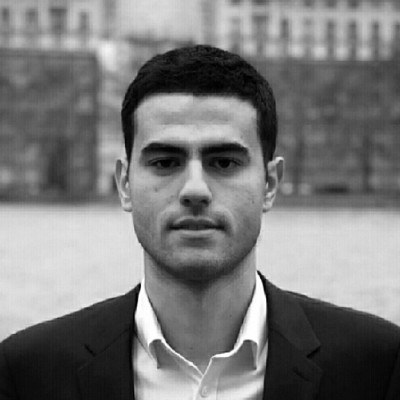
\includegraphics[width=1in,height=1.25in,clip,keepaspectratio]{png/papad}}]{Frixos Papadopoulos}
received the BSc degree in Computer Science from the Department of Electronics and Computer Science, University of Southampton in 2020. He is a prospective postgraduate student in machine learning and his research interests are machine learning and bioinformatics.
\end{IEEEbiography}
% or if you just want to reserve a space for a photo:

\begin{IEEEbiography}{Ashley I. Heinson}
conducted his PhD in the field of Reverse Vaccinology and is currently working as a research fellow in immuno-oncology bioinformatics and predictive modelling at the University of Southampton. Ashley has specialised in RNA-Sequencing analysis but has maintained an interest in machine learning and reverse vaccinology throughout his research.
\end{IEEEbiography}

\begin{IEEEbiography}{Mahesan Niranjan}
received the B.Sc. degree from the University of Peradeniya, Sri Lanka, in 1982, the M.E.E. degree from Eindhoven University of Technology, The Netherlands, in 1985, both in electronic engineering, and the PhD degree from the University of Cambridge, Cambridge, UK, in 1990. He is currently Professor of Electronics and Computer Science at the University of Southampton, Southampton, UK, where he was Head of the Information: Signals, Images and Systems (ISIS) research group. Prior to this appointment in February 2008, he has held a professorship in the University of Sheffield (1999-2008) and a lectureship in the University of Cambridge (1990-1998). At the University of Sheffield, he served as Head of Computer Science (2002-2004) and Dean of the Faculty of Engineering (2006-2008). His research interests are in the algorithmic and applied aspects of machine learning, and he has authored or coauthored about 100 papers in peer-reviewed journals and conferences. He has been Program Chair of several international workshops and has acted as a co-organiser of a six month program on neural networks and machine learning at the Isaac Newton Institute for Mathematical Sciences, Cambridge, UK. His current research has a strong focus on computational biology and biomedical signal processing.
\end{IEEEbiography}

% insert where needed to balance the two columns on the last page with
% biographies
%\newpage

% You can push biographies down or up by placing
% a \vfill before or after them. The appropriate
% use of \vfill depends on what kind of text is
% on the last page and whether or not the columns
% are being equalized.

%\vfill

% Can be used to pull up biographies so that the bottom of the last one
% is flush with the other column.
%\enlargethispage{-5in}


\end{document}


%EXTRA NOTES FROM TEMPLATE CREATOR

%\subsection{Subsection Heading Here}
%Subsection text here.
% needed in second column of first page if using \IEEEpubid
%\IEEEpubidadjcol
%\subsubsection{Subsubsection Heading Here}
%Subsubsection text here.

% An example of a floating figure using the graphicx package.
% Note that \label must occur AFTER (or within) \caption.
% For figures, \caption should occur after the \includegraphics.
% Note that IEEEtran v1.7 and later has special internal code that
% is designed to preserve the operation of \label within \caption
% even when the captionsoff option is in effect. However, because
% of issues like this, it may be the safest practice to put all your
% \label just after \caption rather than within \caption{}.
%
% Reminder: the "draftcls" or "draftclsnofoot", not "draft", class
% option should be used if it is desired that the figures are to be
% displayed while in draft mode.
%
%%\begin{figure}[!t]
%\centering
%\includegraphics[width=2.5in]{myfigure}
% where an .eps filename suffix will be assumed under latex, 
% and a .pdf suffix will be assumed for pdflatex; or what has been declared
% via \DeclareGraphicsExtensions.
%\caption{Simulation results for the network.}
%\label{fig_sim}
%\end{figure}

% Note that the IEEE typically puts floats only at the top, even when this
% results in a large percentage of a column being occupied by floats.
% However, the Computer Society has been known to put floats at the bottom.
